
\part[Estrutura de dados n-dimensionais homogêneas]
{Estrutura de dados n-dimensionais homogêneas}


\chapter[Vetores]
{Vetores}



\section*{Resumo}

Vetores são um tipo de estrutura que podem armazenar um tamanho fixo de elementos do mesmo tamanho e mesmo tipo, alocados em memória contígua. Utiliza-se vetores como um tipo de lista unidimensional, acessada através de índices.


%\begin{chapreferences}{1.}
%\bibliography{playcb}
%\bibliographystyle{plain}
%\nocite{cbook}
%\nocite{sb6}
%\nocite{glfw}
%\nocite{cppbook}

%\end{chapreferences}

% \begin{chapreferences}{1}

% \bibitem{sb6}
% {\em OpenGL SuperBible}.
% \newblock Pearson Education Inc, 6 edition, 2014.

% \bibitem{glfw}
% Marcus Geelnard and Camilla Berglund.
% \newblock {\em GLFW - Reference guide}, 2010.
% \newblock API version 2.7.

% \bibitem{cbook}
% Brian~W. Kernighan and Dennis~M. Ritchie.
% \newblock {\em The C Programming Language}.
% \newblock 1989.

% \bibitem{cppbook}
% Stanley~B. Lippman, Josés Lajoile, and Barbara Moo.
% \newblock {\em C++ Primer}.
% \newblock 2013.
% \end{chapreferences}

\section*{Pré-requisitos}

As práticas deste capítulo exigem que sejam utilizadas as funções
\begin{itemize}
  \item 
    \begin{lstlisting}[language=C++]
    void MudaLimitesJanela(int limite)
    \end{lstlisting}

  \item
    \begin{lstlisting}[language=C++]
    int CriaGrafico(short int index, Ponto *p, int verTipo)
    \end{lstlisting}
\end{itemize}


\section*{Problemas}

\begin{enumerate}
\item
  Exiba o gráfico do polinômio $-x^3$ para $-50 \leq x \leq 50$.
  \label{ex:cap02_ex1}

  \begin{figure}[ht]
    \centerline{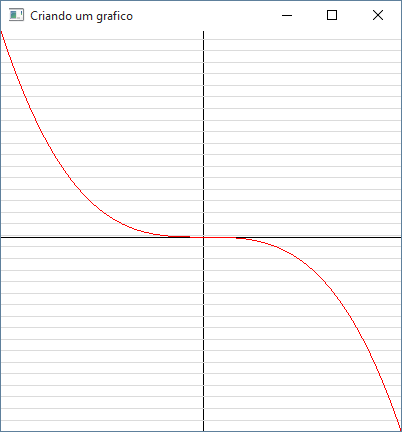
\includegraphics[width=.5\textwidth]{img/cap2_ex8.png}}
    \caption{Gráfico do polinômio $-x^3$}
    \label{fig:cap02_ex1}
  \end{figure}

\item
  Escreva uma programa que solicita ao usuário 20 componentes RGB do tipo int entre 0 e 255 que são armazenadas em três vetores R, G e B. Em seguida, os valores de cada vetor são filtrados por meio da filtragem de média móvel central, como indica a Equação \ref{eq:filtro} e o resultado é armazenado em três novos vetores Rf, Gf, Bf. O tamanho da janela de filtragem é fixo e igual a 3. 

  \label{ex:cap02_ex26}

\begin{equation} \label{eq:filtro}
\begin{matrix}
Rf[i] = & \frac{R[i-1] + R[i] + R[i+1]}{3}\\ 
Gf[i] = & \frac{G[i-1] + G[i] + G[i+1]}{3}\\ 
Bf[i] = & \frac{B[i-1] + B[i] + B[i+1]}{3}
\end{matrix}
\end{equation}
\equationset{Filtragem dos componentes \emph{RGB} do componente \emph{i} com janela de filtragem igual a 3}

  Exiba graficamente dois vetores coloridos, um composto pelas componentes RGB originais e outro pelas componentes RfGfBf filtradas. No final, o programa deve calcular também a distância euclidiana média entre os dois vetores RGB e RfGfBf, como indica a Equação \ref{eq:distancia}.

  \begin{equation} \label{eq:distancia}
  \frac{1}{n}\sum_{i = 0}^{n}\sqrt{(R[i] - Rf[i])^{2} + (G[i] - Gf[i])^{2} + (B[i] - Bf[i])^{2}}
\end{equation}
\equationset{Cálculo da distância euclidiana média}

\begin{figure}[ht]
    \centerline{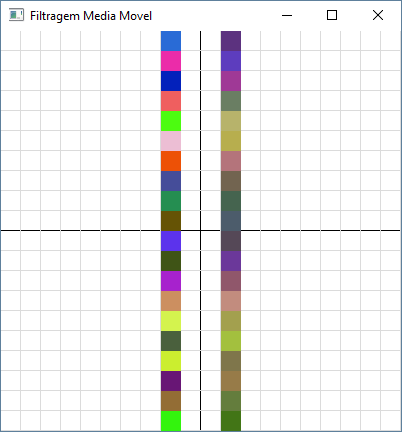
\includegraphics[width=.5\textwidth]{img/cap2_ex26.png}}
    \caption{À esquerda, 20 quadrados com componentes RGB fornecidos pelo usuário. À direita, aplicação do filtro de média móvel central em cada quadrado}
    \label{fig:cap02_ex26}
  \end{figure}


\end{enumerate}

\section*{Soluções}

\subsection*{Exercício \ref{ex:cap02_ex1}}

Esta prática mostra como construir um gráfico a partir de um vetor de Pontos. Cada posição em \emph{y} de cada ponto é calculada dentro do loop. Por padrão, os limites da janela de exibição da playCB vão de -100 à 100, entretanto, os valores em \emph{y} nesta função variam de $-125.000$ até $125.000$, tendo a necessidade de mudar o limite de exibição com a função \emph{MudaLimitesJanela(125000)}.
\lstinputlisting[caption=Código fonte do polinômio, style=customc, label=lst:cap2_ex1]{src/ex8_grafico.cpp}

\begin{lstlisting}[label={func:MudaLimitesJanela},language=C++]
void MudaLimitesJanela(int limite);
\end{lstlisting}
A função \emph{MudaLimitesJanela}, na linha \ref{line:MudaLimitesJanela}, muda o limite da visualização do plano cartesiano, indo de valores $-limite$ até $limite$, tanto em $x$ quanto em $y$. Esta função deve ser chamada antes da função \emph{AbreJanela}.

\begin{lstlisting}[label={func:CriaGrafico},language=C++]
int CriaGrafico(short int index, Ponto *p, short int verTipo);
\end{lstlisting}
A função \emph{CriaGrafico}, na linha \ref{line:CriaGrafico}, cria uma geometria do tipo \emph{GRAFICO}, retornando um índice deste tipo de geometria. A partir de um vetor de pontos \emph{p} de tamanho \emph{index}, esta função cria uma sequência de retas que ligam cada ponto definido pelo vetor. O seu terceiro argumento, \emph{verTipo}, se refere o modo de visualização do gráfico, recebendo os parâmetros descritos na Tabela \ref{tab:CriaGrafico}.

\begin{table}[H]
  \caption{Valor de \emph{verTipo} da função \emph{CriaGrafico}}
  \centering
    \begin{tabular}{lcccc}
    \hline
    Valor&\bf Descrição \\
    \hline
    0 & Não redimensiona a tela  \\
    1  & Redimensiona a tela a fim de comportar toda a função dentro da janela de renderização \\
    2  & Redimensiona a tela a fim de comportar toda a função dentro da janela de rendedização  \\ & sem interferir na escala de ambos os eixos \\
    \hline
  \end{tabular}
  \label{tab:CriaGrafico}
\end{table}

\subsection*{Exercício \ref{ex:cap02_ex26}}

Esta prática exercita conceitos de processamento de imagens, aplicando um filtro dado os componentes RGB da figura, além de exercitar conceitos teóricos de matemática, como o funcionando do operador $\sigma$

\lstinputlisting[caption=Código fonte do filtro de média móvel central, style=customc, label=lst:cap2_ex26]{src/ex26_rgb.cpp}

\chapter[Matrizes]
{Matrizes}



\section*{Resumo}

Assim como vetores, matrizes são um tipo de estrutura que armazena dados de mesmo tamanho e mesmo tipo, mas são utilizadas de maneira n-dimensional. O modo mais comum de utilizar matriz é usando-a na forma bidimensional, onde os dados são tratados como se estivessem numa tabela, com linhas e colunas.


%\begin{chapreferences}{1.}
%\bibliography{playcb}
%\bibliographystyle{plain}
%\nocite{cbook}
%\nocite{sb6}
%\nocite{glfw}
%\nocite{cppbook}

%\end{chapreferences}

% \begin{chapreferences}{1}

% \bibitem{sb6}
% {\em OpenGL SuperBible}.
% \newblock Pearson Education Inc, 6 edition, 2014.

% \bibitem{glfw}
% Marcus Geelnard and Camilla Berglund.
% \newblock {\em GLFW - Reference guide}, 2010.
% \newblock API version 2.7.

% \bibitem{cbook}
% Brian~W. Kernighan and Dennis~M. Ritchie.
% \newblock {\em The C Programming Language}.
% \newblock 1989.

% \bibitem{cppbook}
% Stanley~B. Lippman, Josés Lajoile, and Barbara Moo.
% \newblock {\em C++ Primer}.
% \newblock 2013.
% \end{chapreferences}

\section*{Pré-requisitos}

As práticas deste capítulo exigem que sejam utilizadas as funções
\begin{itemize}
  \item 
    \begin{lstlisting}[language=C++]
    void ExtraiRGBdeBMP(const char *imagepath, int largura, int altura, 
      int (&R)[tam_x][tam_y], int (&G)[tam_x][tam_y], int (&B)[tam_x][tam_y])
    \end{lstlisting}
 
\end{itemize}

\section*{Problemas}
\begin{enumerate}
\item
  Mostre graficamente o jogo da vida para uma matriz com 17 linhas e 17 colunas com a seguinte população inicial onde a população inicial estará \emph{VIVA} para as seguintes posições na matriz:
  $$
    (1,5), (2,5), (3,5), (3,6), (5,1), (5,2), (5,3), (5,6), (5,7), (6,3), (6,5), (6,7), (7,5), (7,6)
  $$
  \label{ex:cap02_ex2}

     \begin{figure*}[!htp]
    \centering
    \begin{subfigure}[t]{0.3\textwidth}
        \centerline{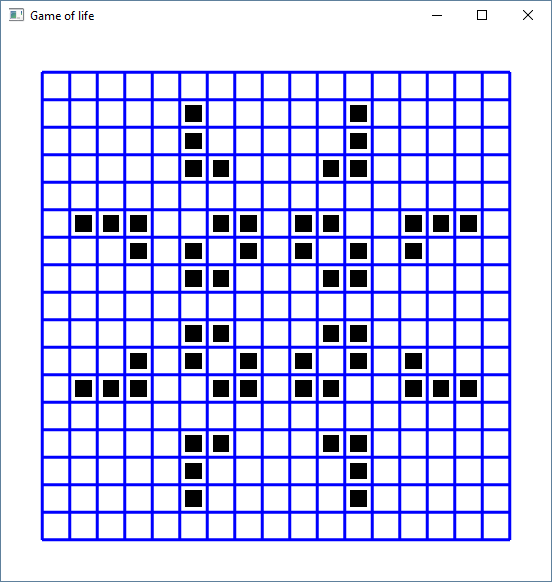
\includegraphics[width=.9\textwidth]{img/cap2_ex9.png}}
        \caption{1ª geração}
        \label{fig:cap03_ex9a}
    \end{subfigure}
    ~
    \begin{subfigure}[t]{0.3\textwidth}
        \centerline{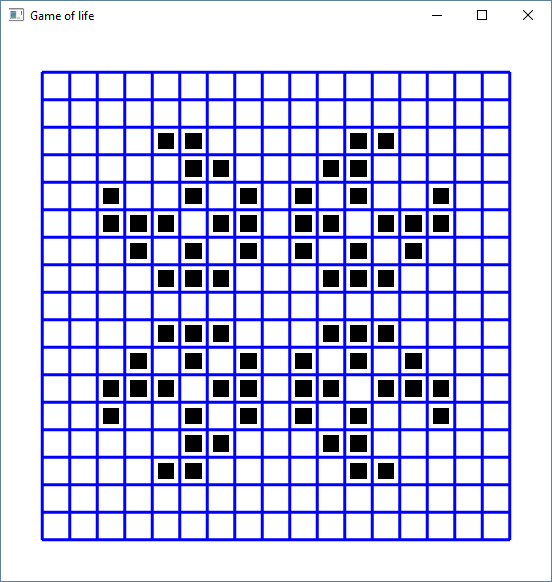
\includegraphics[width=.9\textwidth]{img/cap2_ex9b.png}}
        \caption{2ª geração}
        \label{fig:cap03_ex9a}
    \end{subfigure}
    ~
    \begin{subfigure}[t]{0.3\textwidth}
        \centerline{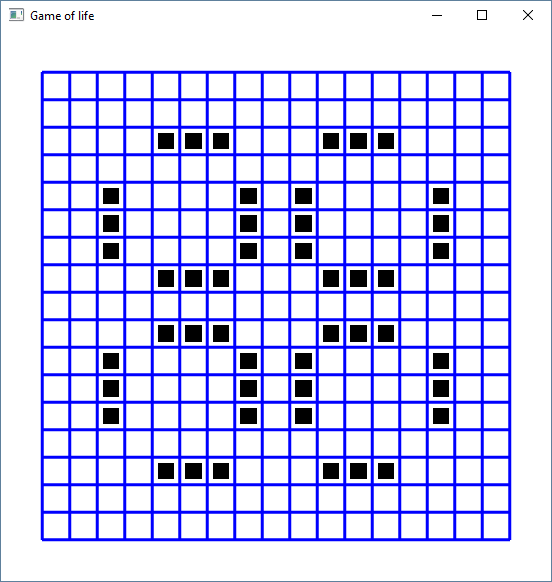
\includegraphics[width=.9\textwidth]{img/cap2_ex9c.png}}
        \caption{3ª geração}
        \label{fig:cap03_ex9a}
    \end{subfigure}
  \end{figure*}

  \item
Implementar o filtro de média móvel para uma matriz M de inteiros (de 0 a 255) com 3 planos RGB, cada um com 100 linhas e 100 colunas.
A matriz a ser filtrada é a imagem uma imagem BMP do Mario. Ela deve ser lida e em seguida mostrada na tela do computador. A imagem filtrada deve igualmente ser apresentada na tela do computador.
  \label{ex:cap02_ex27}

  \begin{figure}[H]
    \centerline{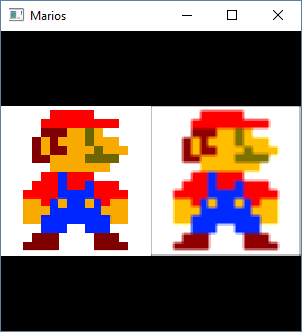
\includegraphics[width=.5\textwidth]{img/cap2_ex27.png}}
    \caption{Filtro Motion Blur}
    \label{fig:cap02_ex27}
  \end{figure}
\end{enumerate}

\section*{Soluções}

\subsection*{Exercício \ref{ex:cap02_ex2}}
Esta prática mostra como utilizar o retorno das função \emph{CriaQuadrado}, que esta retorna o índice da geometria criada. O seu índice é utilizado na função \emph{Pintar}, que recebe, além do índice, o tipo da geometria. Como foi utilizado a função \emph{CriaQuadrado}, o tipo de geometria é \emph{QUADRADO}. Se fosse utilizado \emph{CriaCirculo}, seria utilizado o tipo \emph{CIRCULO} e assim sucessivamente.
\lstinputlisting[caption=Código fonte do jogo da vida, style=customc, label=lst:cap2_ex2]{src/ex9_gameoflife.cpp}

\begin{lstlisting}[label={func:Pintarm2},language=C++]
void Pintar(int red, int green, int blue) 
void Pintar(int red, int green, int blue, geometrias_validas nome, int index)
\end{lstlisting}
A função \emph{Pintar}, na linha \ref{line:Pintarm2} pode ser utilizada de duas formas. No caso da Listagem \ref{lst:cap2_ex2}, como cada índice do tipo \emph{QUADRADO} está salvo na matriz \emph{geoIndex}, na linha \ref{line:matrizgeoIndex}, este índice é passado para o quinto argumento da função \emph{Pintar}. Desta forma, apenas aquela geometria com o valor daquele índice será pintada com as cores especificadas pelos valores \emph{red, green e blue}. O quarto argumento é justamente o tipo de geometria, podendo variar de acordo com a função \emph{Cria} utilizado. A outra forma de utilizar esta função está ilustrada na Listagem \ref{lst:cap1_ex2}.
De forma resumida, o argumento \emph{nome}, do tipo \emph{geometrias\_validas}, pode receber os valores descritos na Tabela ~\ref{tab:PintarM2}.

\begin{table}[H]
  \caption{Valor de \em{nome} da função \em{Pintar}}
  \centering
    \begin{tabular}{lc}
    \hline
    Valor&\bf Retorno da função \\
    \hline
    CIRCULO & CriaCirculo  \\
    QUADRADO  & CriaQuadrado \\
    CIRCUNFERENCIA  & CriaCircunferencia \\
    RETANGULO  & CriaRetangulo \\
    ELIPSE  & CriaElipse \\
    GRAFICO  & CriaGrafico \\
    PONTO  & CriaPonto \\
    RETA  & CriaReta \\
    POLIGONO  & CriaPoligono e CriaPoligonoVetor \\
    TRIANGULO  & CriaTriangulo \\
    \hline
  \end{tabular}
  \label{tab:PintarM2}
\end{table}

\subsection*{Exercício \ref{ex:cap02_ex27}}
Esta prática, assim como o exercício \ref{ex:cap02_ex26}, exercita conceitos de processamento de imagens, com manipulação de componentes RGB, agora distribuídos em uma matriz. Os componentes RGB são extraídos de uma imagem bitmap de 24 bits, e sua visualização também é similar ao exercício \ref{ex:cap02_ex26}.

\lstinputlisting[caption=Código fonte do filtro motion blur, style=customc, label=lst:cap2_ex27]{src/ex27_mario_filtrado.cpp}

\begin{lstlisting}[label={func:ExtraiRGBdeBMP},language=C++]
void ExtraiRGBdeBMP(const char *imagepath, int largura, int altura, 
  int (&R)[tam_x][tam_y], int (&G)[tam_x][tam_y], int (&B)[tam_x][tam_y])
\end{lstlisting}

A função \emph{ExtraiRGBdeBMP}, na linha \ref{line:ExtraiRGBdeBMP}, extrai os componentes RGB de uma imagem e retorna nas matrizes R, G e B. Seu primeiro argumento é o caminho da imagem, o segundo e o terceiro argumento se referem as dimensões da imagem, largura e altura, o quarto, quinto e sexto argumento são as matrizes que irão receber os componentes da imagem, respectivamente R, G e B.
